\documentclass[11pt,a4paper]{article}
\usepackage[utf8]{inputenc}
\usepackage{color}
\usepackage{enumerate}
\usepackage{fancyhdr}
%\usepackage{minted}
\usepackage{graphicx}
\usepackage{array}
\usepackage{hyperref}
\usepackage{amssymb}
\usepackage{multirow}
\usepackage{morefloats}
\usepackage{amsmath}
\usepackage{titlesec}
\usepackage[spanish]{babel}
\usepackage[spanish]{algorithm2e}
\usepackage[table]{xcolor}
\usepackage{anysize}
\usepackage[section]{placeins}
\usepackage{graphicx}
\usepackage{mathtools}
\usepackage{amsmath}


\hypersetup{
	colorlinks,
	citecolor=black,
	filecolor=black,
	linkcolor=black,
	urlcolor=blue
}

\newcommand{\horrule}[1]{\rule{\linewidth}{#1}}

\title{
	\normalfont \normalsize 
	\textsc{\textbf{Metaheurísticas (2016-2017)} \\ Grado en Ingeniería Informática \\ Universidad de Granada} \\ [25pt] % Your university, school and/or department name(s)
	\horrule{0.5pt} \\[0.4cm] % Thin top horizontal rule
	\huge Práctica 1.A: Técnicas de Búsqueda basadas en Poblaciones para el Problema de la Asignación Cuadrática  \\ % The assignment title
	\horrule{2pt} \\[0.5cm] % Thick bottom horizontal rule
}

\author{Germán González Almagro} % Nombre y apellidos

\marginsize{3cm}	% margen izquierdo
{3cm}				% margen derecho
{1.5cm}				% margen superior
{2cm} 			% margen inferior

%\titleformat{\section}{\normalfont\LARGE}{}{0pt}{\bfseries\LARGE}

\begin{document}
	
	\date{\today}
	
	\maketitle
	
	\begin{figure}[!h]
		\centering
		
\includegraphics[scale=0.35]{LogoUGR.png} 
	\end{figure}
	
	\noindent DNI: 76593910T\\Correo Electrónico: germang.almagro@correo.ugr.es\\Subgrupo de prácticas 3. Horario: Lunes de 5:30 a 7:30
	
	\vspace{1cm}
	
	\noindent Algoritmos Considerados: Algoritmo Voraz, Búsqueda Local, Algoritmo Genético Generacional con operadores de cruce de Posición y OX, Algoritmo Genético Estacionario con operadores de cruce de Posición y OX, Algoritmo Memético de mejora completa, Algoritmo Memético de mejora parcial aleatoria, Algoritmo Memético de mejora elitista.
	
	
	\newpage
	
	\tableofcontents
	
	\listoffigures
	
	\listoftables
	
	\newpage
	
\section{Descripción del problema}

	\noindent El problema de la asignación cuadrática o QAP (Quadratic Assignement Problem) es un problema de optimización combinatoria que pertenece a la clase de problemas NP-Completos. Consiste en determinar la asignación óptima de $n$ unidades funcionales a $n$ localizaciones, conociendo el flujo que circula entre cada unidad funcional y la distancia entre las localizaciones.\\
	
	\noindent Para representar este problema de forma que sea computable, consideraremos las matrices $F$ y $D$, que almacenarán el flujo entre unidades y la distancia entre localizaciones respectivamente. De esta manera el flujo entre las unidades $i$ y $j$ es $F_{ij}$ y la distancia entre las localizaciones $k$ y $l$ es $D_{kl}$; el coste de asignar la unidad $i$ a la localización $k$ y la unidad $j$ a la localización $l$ es $F_{ij} \times D_{kl}$.\\
	
	\noindent Conociendo la representación del problema, podemos plantearlo como:
	
	$$ QAP = min \left( \sum_{i=1}^{n}\sum_{j=1}^{n}F_{ij} \times D_{S(i)S(j)} \right)\; t.q.\; S \in \prod_{N} $$
	
\section{Métodos de resolución del problema}

	\noindent Dado que es computacionalmente costoso resolver este problema de forma óptima mediante algoritmos puramente deterministas, emplearemos diversas técnicas heurísticas para obtener una solución que, aunque no es óptima, es de calidad. Las técnicas que emplearemos para ello serán técnicas basadas en poblaciones que evolucionarán de distinta manera, a saber: Algoritmo Genético Generacional con cruce basado en Posición, Algoritmo Genético Generacional con cruce OX, Algoritmo Genético Estacionario con cruce basado en Posición, Algoritmo Genético Estacionario con cruce basado en OX, Algoritmo Memético de mejora completa, Algoritmo Memético de mejora parcial aleatoria, Algoritmo Memético de mejora parcial elitista.\\
	
	\noindent Abordaremos también el problema con técnicas más simples, como pueden ser la Búsqueda Local o la resolución mediante algoritmo Greedy.\\
	
	\noindent Aunque las diferentes técnicas de resolución presentan diferencias significativas, también presentan similitudes; una de ellas es la representación del problema. Las soluciones al problema estarán representadas por una estructura que contendrá un vector que almacena la permutación propuesta como solución, en el que los índices representan las unidades funcionales y el contenido las localizaciones asociadas, además contendrá un dato de tipo \texttt{int} que representa el valor asociado a la permutación propuesta. Entenderemos por dimensión del problema del número de unidades funcionales o localizaciones que lo conforman.
	
	\noindent De igual forma que las diferentes técnicas de resolución comparte el modelo de representación, los algoritmos que las implementan utilizan procesos comunes que pueden ser definidos de forma modular como sigue:
	
	\newpage
	
	\subsection{Función objetivo}
	
		\noindent La función objetivo es la encargada de dar valor al campo de tipo \texttt{int} asociado a una solución, para ello, recorre la matriz de distancias y de flujo realizando las operaciones pertinentes sobre un acumulador.
		
		\begin{algorithm}
			\KwIn{Dada una solcuión $S$}
			\textbf{function} $CalcularSolucionNumerica(\&S)$
			\Begin{
				$SNumerica \leftarrow 0$\\
				\For{$i \leftarrow 0$ \KwTo $Dimension$}{
					\vspace{0.2cm}
					\For{$j \leftarrow 0$ \KwTo $Dimension$}{
						\vspace{0.2cm}
						$SNumerica \leftarrow SNumerica + MatrizFlujo_{ij} \times$\\ $MatrizDistancias_{S_i,S_j}$		
					}
				}
				$S.SolucionNumerica \leftarrow SNumerica$
			}
			
		\end{algorithm}
	
	\subsection{Factorización de la función objetivo}
	
		\noindent Es posible reducir el esfuerzo computacional realizado al evaluar un individuo de forma que, conociendo el estado del mismo, a saber, permutación que almacena y valor numérico de la misma, factorizamos el cálculo del coste de forma que el orden de complejidad del algoritmo que lo calcula se reduce de $\mathcal{O}(n^2)$ a $\mathcal{O}(n)$.			
		
		\begin{algorithm}
			\KwIn{Dados $s$ y $r$ las posiciones a intercambiar y $\pi$ la solución}
			\textbf{function} $ChequearMovimiento(s,\; r,\; \pi)$
			\Begin{
				$Incremento \leftarrow 0$\\
				\For{$k \leftarrow 0$ \KwTo $Dimension$}{
					\vspace{0.2cm}
					\If{$k \neq s$ $\&\&$ $k \neq r$}{
						
						$Incremento \leftarrow Incremento + F_{rk}(D_{\pi(s)\pi(k)} - D_{\pi(r)\pi(k)}) +$\\
						$F_{sk}(D_{\pi(r)\pi(k)} - D_{\pi(s)\pi(k)}) +$\\
						$F_{kr}(D_{\pi(k)\pi(s)} - D_{\pi(k)\pi(r)}) +$\\
						$ F_{ks}(D_{\pi(k)\pi(r)} - D_{\pi(k)\pi(s)})$
						
					}		
				}
				
				\KwRet $Incremento$
			}
			
		\end{algorithm}
		
		\noindent Dado que, tanto el orden de complejidad como el espacio de trabajo de la función objetivo y su versión factorizada no es el mismo, es lógico pensar que no deben contabilizar de igual forma para la obtención del número total de llamadas a la función objetivo que realiza un algoritmo. Como ya hemos visto, mientras que le orden de complejidad de la función objetivo es $\mathcal{O}(n^2)$, el de su versión factorizada es de orden $\mathcal{O}(n)$, concretamente $\mathcal{O}(4n)$, por tanto para completar una llamada a la función objetivo empleando únicamente llamadas a la función factorizada será necesario realizar $\frac{N}{4}$ llamadas a la misma.
		
	\subsection{Operador de mutación y generación de vecinos}
	
		\noindent Dado que el vecindario de una solución está compuesto por todas aquellas soluciones que presenten diferencia únicamente en dos de los índices asociados a la permutación que las conforman, es sencillo definir el operador que genera un vecino a partir de una solución. Basta con hacer uso de la función objetivo factorizada, para obtener el incremento o decremento del valor numérico de la solución, para poder así sumarlo al valor numérico del vecino generado, e intercambiar las dos posiciones que dan lugar a esta modificación del valor.
	
		\begin{algorithm}
			\textbf{function} $GenerarVecino/Mutar(i,\;j,\;\&Solucion)$
			\Begin{
				
				$Incremento \leftarrow CheckMove(i,\;j,\;Solucion)$\\
				$Solucion.IntercambiarIndices(i,\;j)$\\
				$Solucion.Valor \leftarrow Solucion.Valor + Incremento$\\
					
			}
			
			
		\end{algorithm}	
			
	\subsection{Generación de soluciones aleatorias}
	
		\noindent Para trabajar con algoritmos basados en poblaciones es necesario contar con una población inicial que, en este caso, estará formada por soluciones factibles aleatorias generadas siguiendo el proceso descrito en el pseudocódigo.
	
		\begin{algorithm}
			
			\textbf{function} $GenerarSolucionAleatoria(\&Solucion)$
			\Begin{
			
				$Solucion \leftarrow \emptyset$\\
				\vspace{0.2cm}
				\For{$i \leftarrow 0$ \KwTo $Dimension$}{
					$Solucion[i] \leftarrow i$\\
							
				}
				
				\texttt{\#Barajamos el vector que contiene la permutación solución}\\
				\For{$i \leftarrow 0$ \KwTo $Dimension$}{
					
					$Rand \leftarrow AleatorioEntre(i,\;Dimension)$\\
					$Solucion.Intercambiar(Rand,\; i)$\\
					
				}
				
				$CalcularSolucionNumerica(Solucion)$\\
			}
			
			
		\end{algorithm}
		
	\subsection{Operador de mutación}
	
	\noindent El operador de mutación es el encargado de introducir diversidad en la población, basta con seleccionar de forma aleatoria cromosomas de la población así como los dos genes que se intercambiarán para hacer efectiva la mutación. Cabe destacar que, el número de mutaciones se calcula como: $NumMutaciones = ProbabilidadMutacion \times NumeroCromosomas \times GenesPorCromosoma$, de esta forma obtenemos el número de genes que mutan, y, puesto que en cada individuo mutan dos genes, el número de individuos que mutan es:\\ $NumeroMutaciones/2$.
	
	\begin{algorithm}
		
		\textbf{function} $AplicarMutacion(\&Poblacion,\;NumMutaciones)$
		\Begin{
			\For{$i \leftarrow 0$ \KwTo $NumeroMutaciones/2$}{
				
				$Crma \leftarrow Poblacion[AleatorioEntre(0,TamPoblacion-1)] $\\
				\vspace{0.2cm}
				\texttt{\#$Gen1$ y $Gen2$ deben ser diferentes}\\
				$Gen1 \leftarrow AleatorioEntre(0,Dimension-1)$\\
				$Gen2 \leftarrow AleatorioEntre(0,Dimension-1)$\\
				\vspace{0.2cm}
				$Mutar(Gen1,\;Gen2,\;Crma)$
			}
		}
		
	\end{algorithm}	
	
	\noindent Cabe destacar que, como veremos mas adelante, el proceso de mutación es el mismo en los algoritmos genéticos estacionarios y generacionales, aunque no la forma en la que esta se aplica.
	
	\subsection{Operador de selección en los Algoritmos Genéticos}
	
		\noindent El mecanismo de selección empleado es el torneo binario, es decir, se seleccionan dos parejas de individuos de la población en las que cada individuo compite con el otro para ser seleccionado como padre. El motivo del uso de este mecanismo de selección es evitar seleccionar soluciones pobres como padres, ya que, para que se seleccionasen como padres dos soluciones pobres debe darse el caso de que las 4 soluciones seleccionadas sean malas soluciones.

		\noindent (Para el correcto funcionamiento de este algoritmo es necesario mantener ordenada la población, así como mantener en memoria un vector que contenga todas las posibles parejas para seleccionar los competidores del torneo; los mecanismos empleados para ello serán detallados más adelante.)\\

		\begin{algorithm} [!h]
			
			\Begin{
				
				\texttt{\\.....}\\
				\For{$i \leftarrow 0$ \KwTo $NumeroCruces$}{
					\vspace{0.2cm}
					$ParejaAleatoria \leftarrow VectorParejas(Rand)$\\
					\vspace{0.1cm}
					$Candidato1 \leftarrow ParejaAleatoria.first$\\
					$Candidato2 \leftarrow ParejaAleatoria.second$\\
					\vspace{0.1cm}
					$Padre1 \leftarrow Candidato1 < Candidato2? Candidato1:Candidato2$\\
					\vspace{0.1cm}
					$ParejaAleatoria \leftarrow VectorParejas(Rand)$\\
					\vspace{0.1cm}
					$Candidato1 \leftarrow ParejaAleatoria.first$\\
					$Candidato2 \leftarrow ParejaAleatoria.second$\\
					\vspace{0.1cm}
					$Padre2 \leftarrow Candidato1 < Candidato2? Candidato1:Candidato2$\\
					\vspace{0.1cm}
					$Hijo \leftarrow OperadorCruce(Padre1,\;Padre2)$\\
					\vspace{0.1cm}
					$NuevosIndividuos \leftarrow NuevosIndividuos \cup Hijo$\\
					\vspace{0.2cm}
					
				}
				
				\texttt{.....}
				
			}
			
			
		\end{algorithm}
		
\newpage
		
	\subsection{Operadores de cruce}
	
		\subsubsection{Operador de cruce basado en posiciones comunes}
	
		\noindent El funcionamiento del operador de cruce basado en posiciones comunes es simple; consiste en asignar a la permutación del hijo los elementos que coincidan en ambos padres y asignar de manera aleatoria el resto en aquellas posiciones de la permutación del hijo no ocupadas ya por elementos comunes.

		\begin{algorithm}
	
			\textbf{function} $OperadorDeCrucePorPosicion(Padre1,\;Padre2)$
			\Begin{
				$Hijo \leftarrow \emptyset\;\;$
				$NoComunes \leftarrow \emptyset$\\
				
				\For{$i \leftarrow 0$ \KwTo $Dimension$}{
					
					\uIf{$Coinciden\; Padre1\; y\; Padre2$}{
						
						$Hijo[i] \leftarrow Padre1[i]$
						
					} 
					
					\Else{
					
						$Hijo[i] \leftarrow ValorEspecial$\\
						$NoComunes.Add(Padre1[i])$
						
					}
				
					
				}
				
		
				$BarajarVector(NoComunes)$

				
				\For{$i \leftarrow 0$ \KwTo $Dimension$}{
					
					
					\If{$Hijo[i]\; contiene\; Valor\; especial$}{
						
						$Hijo[i] \leftarrow NoComunes[Elemento]$
					}
					
					
				}
				$CalcularSolucionNumerica(Hijo)$\\
				\KwRet $Hijo$
			
			}
			
		\end{algorithm}
		
\newpage
	
	\subsubsection{Operador de cruce OX}
	
		\noindent Consiste en seleccionar un segmento de alguno de los padres que será copiado en el hijo sin modificación, todos aquellos elementos de la permutación del padre seleccionado como portador del segmento que hayan quedado fuera del mismo serán copiados en el hijo, en las posiciones vacías, atendiendo al orden en el que aparecen en el segundo padre.

		\begin{algorithm} [!h]
			
			\textbf{function} $OperadorDeCruceOX(Padre1,\;Padre2)$
			\Begin{
				$Segmento \leftarrow Dimension \times 0.45$\\
				$Inicio \leftarrow Dimension/2 - Segmento/2$\\
				$Fin \leftarrow Inicio + Segmento\;$
				$Hijo \leftarrow \emptyset\;\;$
				$NoSegmento \leftarrow \emptyset$\\
				
				\For{$i \leftarrow 0$ \KwTo $Dimension$}{
				
					\uIf{$i \in [Inicio,Fin)$}{
						
						$Hijo[i] \leftarrow Padre1[i]$
						
					} 
					
					\Else{
						
						$NoSegmento.Add(Padre1[i])$
						
					}
					
				}
				
				
				 \texttt{\#Ordenamos los elementos del vector atendiendo al orden en el que aparecen en $Padre2$} \\
				$OrdenarSegunPadre2(NoSegmento)$\\
				
				
				\For{$i \leftarrow 0$ \KwTo $Dimension$}{
					
					\uIf{$i \notin [Inicio,Fin)$}{
						$Hijo[i] \leftarrow NoSegmento[Elemento]$\\
						$Elemento++$
					} 
					
				}
				
				$CalcularSolucionNumerica(Hijo)$\\
				
				\KwRet $Hijo$
				
			}
			
		\end{algorithm}	
		
\newpage
\section{Algoritmo de Búsqueda Local}

	\noindent En esta ocasión, emplearemos, para la implementación de la búsqueda local, un vector que nos permitirá ``guiar'' el proceso de búsqueda de forma que evitamos explorar ramas que sabemos que no conducen a una buena solución, el vector Don't look bits (DLB). El esquema general consiste en generar vecinos de una solución de manera aleatoria, para no dar prioridad a unos sobre otros, de forma que la solución actual será reemplazada por el primer vecino que proporcione una mejora a la solución. A continuación se muestra el pseudocódigo del método descrito. (Suponer que las operaciones se realizan sobre una interna a la clase).

	\begin{algorithm} [!h]
		
		\textbf{function} $BusquedaLocal(MaxLlamadas)$
		\Begin{
			
			$Intercamb \leftarrow Solucion \leftarrow PermutacionAleatoria$\\
			
			
			\While{$Se\; ha\; producido\; mejora\; \&\&\; Llamadas\; <\; MaxLlamada$}{
				
				$BarajarVector(Intercamb)$\\
				$DLB \leftarrow \{0\}$	
				
				\For{$(i \leftarrow 0$; $\;i<Dimension\; \&\&\; No Mejora$; $\;i++)$}{
					
					\uIf{$DLB[i] == 0$}{
						
						\For{$(i \leftarrow 0$; $\;i<Dimension\; \&\&\; No Mejora$; $\;i++)$}{
							
							$Incremento \leftarrow ChequearMovimiento(Intercamb[i],Intercamb[j])$\\
							$Llamadas \leftarrow Llamadas + 1/(Dimension/4)$
							
							\uIf{$Incremento < 0$}{
								
								$Individuo \leftarrow Vecino$\\
								$Llamadas \leftarrow Llamadas + 1/(Dimension/4)$\\
								$DLB[Intercamb[i]] \leftarrow DLB[Intercamb[j]] \leftarrow 0$
								
							}
							\Else{
								
								$DLB[Intercamb[i]] \leftarrow 1$
							
							}
							
							
						}
						
					} 
					
				}
				
			}
			
			
		}
		
	\end{algorithm}

\newpage
	
\section{Algoritmos Genéticos Generacionales}

	\noindent Los algoritmos genéticos generacionales son métodos de exploración de espacios de soluciones basados en poblaciones en los que, en cada iteración, se genera una población de tamaño igual a la anterior de forma que la nueva población reemplaza por completo a la siguiente, a excepción del mejor elemento de la población anterior, en caso de que este sea mejor que el nuevo mejor individuo generado.\\
	
	\noindent Para el correcto funcionamiento de este algoritmo es necesario mantener ordenada la población, pero, dado que sería muy costoso computacionalmente ordenar un vector de vectores que pueden ser de gran tamaño, mantendremos ordenada una estructura auxiliar en la que almacenamos parejas formadas por: el índice asociado a cada individuo en el vector de población y el valor de la solución asociada al mismo. De esta forma no es necesario ordenar la población, bastará con ordenar la estructura descrita atendiendo al valor de cada solución. Una de las ventajas de este método es que el torneo binario es inmediato, puesto que bastará con seleccionar al azar dos individuos del vector ordenado y comparar sus índices, aquel cuyo índice sea menor será seleccionado.\\
	
	\noindent Otro aspecto importante a tener en cuenta es que, el proceso de generación de números aleatorios consume tiempo de ejecución, por tanto, reducir el número de llamadas al generador de números aleatorios proporcionará una mejora en el tiempo de ejecución. Por este motivo mantendremos en memoria un vector de parejas que contendrá todas las posibles parejas (no repetidas) de números enteros comprendidos en el intervalo $[0,Dimension)$ donde la dimensión es el tamaño de la permutación. De esta forma basta con generar un único número aleatorio para llevar a cabo los torneos binarios, en lugar de los dos que serían necesarios en caso de no utilizar este mecanismo.\\
	
	\noindent Dado que el número de individuos generados en cada iteración viene dado por una probabilidad de cruce, y es calculado como $NumNuevosIndividuos = TamanioPoblacion \times ProbabilidadCruce$, es posible que no se generen tantos individuos como tamaño tenga la población completa. Puesto que el tamaño de la población debe ser constante a lo largo del proceso de evolución, puede ser necesario conservar miembros de la $Iteracion_{t-1}$ en la iteración $Iteracion_{t}$, en este caso, se conservarán los mejores individuos.\\
	
	\noindent La única diferencia entre el algoritmo genético generacional con operador de cruce por posición y con operador de cruce OX es la llamada la función que genera el hijo dados dos padres.
	
	\newpage
	
		\begin{algorithm} [!h]
			
			\textbf{function} $AGG-Posicion/OX(Pc, Pm, MaxEvals, TamanioPoblacion)$
			\Begin{
				\texttt{\# Cáculo del número de cruces a realizar}\\
				$NumCruces \leftarrow TamanioPoblacion \times Pc)$\\
				\texttt{\# Cáculo del número de mutaciones a realizar}\\
				$NumMutaciones \leftarrow Pm \times TamanioPoblacion \times Dimension$\\
				\vspace{0.2cm}
				\texttt{\#Inicializamos una población aleatoria de tamaño $TamanioPoblacion$ }\\
				$InicializarPoblacionAleatoria(TamanioPoblacion)$\\
				\texttt{\#Inicializar y ordenar el vector que indica el orden de la población}\\
				$Inicializar(OrdenPoblacion)$\\
				$Ordenar(OrdenPoblacion)$\\
				$Evals \leftarrow 0$
					
				\While{$Evals\; <\; MaxEvals$}{
					
					$NuevosIndividuos \leftarrow \emptyset$\\
					
					\For{$i \leftarrow 0$ \KwTo $NumCruces$}{
						\vspace{0.2cm}
						$ParejaAleatoria \leftarrow VectorParejas(Rand)$\\
						\vspace{0.1cm}
						$Candidato1 \leftarrow ParejaAleatoria.first$\\
						$Candidato2 \leftarrow ParejaAleatoria.second$\\
						\vspace{0.1cm}
						$Padre1 \leftarrow Candidato1 < Candidato2? Candidato1:Candidato2$\\
						\vspace{0.1cm}
						$ParejaAleatoria \leftarrow VectorParejas(Rand)$\\
						\vspace{0.1cm}
						$Candidato1 \leftarrow ParejaAleatoria.first$\\
						$Candidato2 \leftarrow ParejaAleatoria.second$\\
						\vspace{0.1cm}
						$Padre2 \leftarrow Candidato1 < Candidato2? Candidato1:Candidato2$\\
						\vspace{0.1cm}
						$Hijo \leftarrow OperadorCrucePosicion/OX(Padre1,\;Padre2)$\\
						\vspace{0.1cm}
						$NuevosIndividuos \leftarrow NuevosIndividuos \cup Hijo$\\
						\vspace{0.2cm}
						
					}
					
					$AplicarMutacion(NuevosIndividuos,\; NumMutaciones)$
					$Evals \leftarrow Evals + NumCruces + NumMutaciones/(Dimension/4)$
					
					\texttt{\#Buscamos el mejor y el peor individuo de entre los generados}
					$MejorIndividuoNuevo \leftarrow BuscarMejor(NuevosIndividuos)$\\
					$PeorIndividuoNuevo \leftarrow BuscarPeor(NuevosIndividuos)$\\
					
					\If{$MejorIndividuoPoblacion < MejorIndividuoNuevo$}{
						
						$NuevosIndividuos.Eliminar(PeorIndividuoNuevo)$\\
						$NuevosIndividuos.Aniadir(MejorIndividuoPoblacion)$\\
				
					}
					
					\texttt{\#Si es necesario añadir individuos, añadimos los mejores de la poblacion anterior}\\
					\If{$NuevosIndividuos.Size() < TamanioPoblacion$}{
					
						$Restantes \leftarrow TamanioPoblacion - NuevosIndividuos.Size()$\\
						
						\For{$i \leftarrow 0$ \KwTo $Restantes$}{
							
							$NuevosIndividuos.Aniadir(Poblacion[OrdenPoblacion[i]])$
							
						}	
						
					}
					
					$Poblacion \leftarrow NuevosIndividuos$\\
					$Inicializar(OrdenPoblacion)$\\
					$Ordenar(OrdenPoblacion)$\\
					
				}
				
				
			}
			
		\end{algorithm}
		
\section{Algoritmos Genéticos Estacionarios}

	\noindent Los algoritmos genéticos estacionarios, de igual forma que los generacionales, son métodos de exploración de espacios de soluciones basados en poblaciones en los que, a diferencia de como se procede en los generacionales, en cada iteración, se generan dos individuos que compiten con los dos últimos individuos de la población para pasar a formar parte de la misma. En caso de que sean mejores, los peores individuos de la población se verán reemplazados por los nuevos individuos.\\
	
	\noindent De igual forma que en los algoritmos generacionales, haremos uso de un vector auxiliar para mantener ordenada la población sin un sobrecoste computacional, así como emplearemos el mismo vector de parejas para seleccionar los competidores para los torneos binarios.\\
	
	\noindent Para determinar si los dos individuos generados reemplazan a los dos últimos de la población, realizamos un torneo que implica a los individuos generados y a los dos últimos individuos de la población. Los dos ganadores de este torneo serán los que reemplacen a los dos últimos individuos de la población. Para realizar el torneo basta con ordenar un vector que contenga a los 4 participantes.\\
	
	\noindent La diferencia más notable se encuentra en el método de mutación, en este caso no es posible aplicar a cada nueva población de individuos un número fijo de mutaciones calculadas en base a un porcentaje, debido al tamaño de la misma, a saber, 2. En su lugar calcularemos la frecuencia esperada con la que un gen muta, a saber, $FrecuenciaMutacion = ((1/ProbabilidadMutacion)/TamPoblacion)$, y contaremos el número de nuevos individuos generados hasta alcanzar dicha frecuencia, en cuyo caso mutaremos uno de los individuos de la población.\\
	
	
		\begin{algorithm} [!h]
			
			\textbf{function} $AGE-Posicion/OX(Pm, MaxEvals, TamPoblacion)$
			\Begin{
				$NumCruces \leftarrow 2)\;\; NumMutaciones \leftarrow 2\;\; ContMut \leftarrow 0$\\
				$FrecuenciaMutacion \leftarrow ((1/ProbabilidadMutacion)/TamPoblacion)$
				\vspace{0.2cm}
				\texttt{\#Inicializamos una población aleatoria de tamaño $TamanioPoblacion$ }\\
				$InicializarPoblacionAleatoria(TamPoblacion)$\\
				\texttt{\#Inicializar y ordenar el vector que indica el orden de la población}\\
				$Inicializar(OrdenPoblacion)$\\
				$Ordenar(OrdenPoblacion)$\\
				$Evals \leftarrow 0$
				
				\While{$Evals\; <\; MaxEvals$}{
					
					$NuevosIndividuos \leftarrow \emptyset$\\
					
					\For{$i \leftarrow 0$ \KwTo $NumCruces$}{
						\vspace{0.2cm}
						$ParejaAleatoria \leftarrow VectorParejas(Rand)$\\
						\vspace{0.1cm}
						$Candidato1 \leftarrow ParejaAleatoria.first$\\
						$Candidato2 \leftarrow ParejaAleatoria.second$\\
						\vspace{0.1cm}
						$Padre1 \leftarrow Candidato1 < Candidato2? Candidato1:Candidato2$\\
						\vspace{0.1cm}
						$ParejaAleatoria \leftarrow VectorParejas(Rand)$\\
						\vspace{0.1cm}
						$Candidato1 \leftarrow ParejaAleatoria.first$\\
						$Candidato2 \leftarrow ParejaAleatoria.second$\\
						\vspace{0.1cm}
						$Padre2 \leftarrow Candidato1 < Candidato2? Candidato1:Candidato2$\\
						\vspace{0.1cm}
						$Hijo \leftarrow OperadorCrucePosicion/OX(Padre1,\;Padre2)$\\
						\vspace{0.1cm}
						$NuevosIndividuos \leftarrow NuevosIndividuos \cup Hijo$\\
						\vspace{0.2cm}
						
					}
					
					$ContMut \leftarrow ContMut + NumCruces$
					\If{$ContMut \ge FrecuenciaMutacion$}{
						$AplicarMutacion(NuevosIndividuos,\; NumMutaciones)$\\
						$Evals \leftarrow Evals + NumCruces + NumMutaciones/(Dimension/4)$\\
					}
					\Else{
						$Evals \leftarrow Evals + NumCruces$
					}
					
					\texttt{\#Añadimos los dos últimos individuos de la población a los generados para realizar el torneo}\\
					$NuevosIndividuos.Add(Poblacion[OrdenPoblacion[TamPoblacion-1]])$\\
					$NuevosIndividuos.Add(Poblacion[OrdenPoblacion[TamPoblacion-2]])$\\
					
					$Ordenar(NuevosIndividuos)$\\
					
					\texttt{\#Sustituimos los dos últimos elementos de la población por los ganadores}\\
					$Poblacion[OrdenPoblacion[TamPoblacion-2]] \leftarrow NuevosIndividuos[0]$\\
					$Poblacion[OrdenPoblacion[TamPoblacion-1]] \leftarrow NuevosIndividuos[1]$\\
					
					$Inicializar(OrdenPoblacion)$\\
					$Ordenar(OrdenPoblacion)$\\
					
				}
				
				
			}
			
		\end{algorithm}
		

\section{Algoritmos Meméticos}

	\noindent Los algoritmos meméticos son algoritmos basados en evolución de poblaciones que utilizan todo el conocimiento disponible sobre el problema para realizar búsqueda heurística. En este caso basaremos los algoritmos meméticos en los algoritmos genéticos generacionales con cruce basado en posición, con la diferencia de que lanzaremos una búsqueda local sobre toda la población o un subconjunto de la misma con cierta frecuencia, antes de generar los nuevos individuos.\\
	
	\noindent Debemos tener en consideración que la búsqueda local realiza llamadas a la función objetivo y a su factorización, por tanto estas llamadas deben computar para el calculo del contador que controla la condición de parada. Además, al aplicar una búsqueda local sobre los individuos de la población es posible que cambie el orden de la misma, por lo que deberemos reordenarla tras aplicar la búsqueda local a la población.
	
	\subsection{Algoritmo Memético de mejora completa (AM - (10, 1.0))}
	
		\noindent En este caso, cada 10 iteraciones, lanzaremos una búsqueda local sobre todos los miembros de la población. Para ello basta con recorrer en un bucle la población y llamar al algoritmo $LocalSearch(\&Solucion)$ sobre cada uno de ellos.\\
		
		\noindent El siguiente pseudocódigo pone de manifiesto las diferencias entre el algoritmo memético y el algoritmo genético generacional:\\
		
		\begin{algorithm} [!h]
			
			\textbf{function} $AMFull(Pc, Pm, MaxEvals, TamanioPoblacion)$
			\Begin{
				\texttt{Declaración de variables...}\\
				$FrecuenciaLS \leftarrow 10\;\;EvalsLS \leftarrow 0\;\; ContadorGeneraciones \leftarrow 0$\\
				\texttt{Inicializar y ordenar $OrdenPoblacion$...}\\
				
				\While{$Evals\; <\; MaxEvals$}{
					
					$NuevosIndividuos \leftarrow \emptyset$\\
					
					\If{$ContadorGeneraciones \ge FrecuenciaLS$}{
						
						$ContadorGeneraciones \leftarrow 0$
						
						\For{$i \leftarrow 0$ \KwTo $TamanioPoblacion$}{
							
							$EvalsLS \leftarrow EvalsLS + LocalSearch(Poblacion[i])$\\
							
						}
						
						\texttt{Reiniciar y ordenar $OrdenPoblacion$...}\\
					
					}
					
					\texttt{Generación de nuevos individuos...}\\
					\texttt{Aplicar mutación...}\\
					$Evals \leftarrow Evals + EvalsLS + NumCruces + NumMutaciones/(Dimension/4)$\\
					\texttt{Conservar Elitismo...}\\
					\texttt{Mantener constante el tamaño de la población...}\\
					
					$Poblacion \leftarrow NuevosIndividuos$\\
					
					\texttt{Reiniciar y ordenar $OrdenPoblacion$...}\\
					
					$ContadorGeneraciones \leftarrow ContadorGeneraciones + 1$
					
				}
				
				
			}
			
		\end{algorithm}
		
		\subsection{Algoritmo Memético de mejora parcial aleatoria (AM - (10, 0.1))}
		
		\noindent En este caso, cada 10 iteraciones, lanzaremos una búsqueda local sobre un subconjunto aleatorio de los miembros de la población. Para no aplicar dos veces la búsqueda local sobre el mismo individuo, mantendremos en memoria un vector que contendrá todos los índices asociados a la población una única vez. Para seleccionar miembros aleatorios de la población barajaremos este vector cada vez que sea necesario.\\
		
		\noindent El siguiente pseudocódigo pone de manifiesto las diferencias entre el algoritmo memético y el algoritmo genético generacional:\\
		
		\begin{algorithm} [!h]
			
			\textbf{function} $AMSub(Pc, Pm, MaxEvals, TamanioPoblacion)$
			\Begin{
				\texttt{Declaración de variables...}\\
				$FrecuenciaLS \leftarrow 10\;\;EvalsLS \leftarrow 0\;\; ContadorGeneraciones \leftarrow 0$\\
				\texttt{\#Declaracion del vector de indices}\\
				$VA \leftarrow \{0...TamanioPoblacion-1\}$\\
				$Barajar(VectorAleatorio)$\\
				$IndiceVA \leftarrow 0$\\
				
				\texttt{Inicializar y ordenar $OrdenPoblacion$...}\\
				
				\While{$Evals\; <\; MaxEvals$}{
					
					$NuevosIndividuos \leftarrow \emptyset$\\
					
					\If{$ContadorGeneraciones \ge FrecuenciaLS$}{
						
						$ContadorGeneraciones \leftarrow 0$
						
						\For{$i \leftarrow 0$ \KwTo $TamanioPoblacion \times 0.1$}{
							
							$EvalsLS \leftarrow EvalsLS + LocalSearch(Poblacion[VA[IndiceVA]])$\\
							$IndiceVA \leftarrow IndiceVA + 1$\\
							
						}
						
						\If{$IndiceVA \ge VA.Size()-1$}{
							$Barajar(VectorAleatorio)$\\
							$IndiceVA \leftarrow 0$\\
						}
						
						\texttt{Reiniciar y ordenar $OrdenPoblacion$...}\\
						
					}
					
					\texttt{Generación de nuevos individuos...}\\
					\texttt{Aplicar mutación...}\\
					$Evals \leftarrow Evals + EvalsLS + NumCruces + NumMutaciones/(Dimension/4)$\\
					\texttt{Conservar Elitismo...}\\
					\texttt{Mantener constante el tamaño de la población...}\\
					
					$Poblacion \leftarrow NuevosIndividuos$\\
					
					\texttt{Reiniciar y ordenar $OrdenPoblacion$...}\\
					
					$ContadorGeneraciones \leftarrow ContadorGeneraciones + 1$
					
				}
				
				
			}
			
		\end{algorithm}
		
		\newpage
		
		\subsection{Algoritmo Memético de mejora elitista (AM - (10, 0.1 mej))}
		
		\noindent En este caso, cada 10 iteraciones, lanzaremos una búsqueda local sobre los $n$ mejores miembros, donde $n = TamanioPoblacion \times 0.1$ .
		
		\noindent El siguiente pseudocódigo pone de manifiesto las diferencias entre el algoritmo memético y el algoritmo genético generacional:\\
		
		\begin{algorithm} [!h]
			
			\textbf{function} $AMElite(Pc, Pm, MaxEvals, TamanioPoblacion)$
			\Begin{
				\texttt{Declaración de variables...}\\
				$FrecuenciaLS \leftarrow 10\;\;EvalsLS \leftarrow 0\;\; ContadorGeneraciones \leftarrow 0$\\
				\texttt{Inicializar y ordenar $OrdenPoblacion$...}\\
				
				\While{$Evals\; <\; MaxEvals$}{
					
					$NuevosIndividuos \leftarrow \emptyset$\\
					
					\If{$ContadorGeneraciones \ge FrecuenciaLS$}{
						
						$ContadorGeneraciones \leftarrow 0$
						
						\For{$i \leftarrow 0$ \KwTo $TamanioPoblacion \times 0.1$}{
							
							$EvalsLS \leftarrow EvalsLS + LocalSearch(Poblacion[OrdenPoblacion[i]])$\\
							
						}
						
						\texttt{Reiniciar y ordenar $OrdenPoblacion$...}\\
						
					}
					
					\texttt{Generación de nuevos individuos...}\\
					\texttt{Aplicar mutación...}\\
					$Evals \leftarrow Evals + EvalsLS + NumCruces + NumMutaciones/(Dimension/4)$\\
					\texttt{Conservar Elitismo...}\\
					\texttt{Mantener constante el tamaño de la población...}\\
					
					$Poblacion \leftarrow NuevosIndividuos$\\
					
					\texttt{Reiniciar y ordenar $OrdenPoblacion$...}\\
					
					$ContadorGeneraciones \leftarrow ContadorGeneraciones + 1$
					
				}
				
				
			}
			
		\end{algorithm}
		
\newpage
		
\section{Algoritmo de comparación: Algoritmo Greedy}

	\noindent Los algoritmos voraces proporcionan soluciones a problemas en tiempo mínimo a costa de una pérdida de calidad en la solución. En este caso el algoritmo voraz consiste en seleccionar iterativamente las unidades funcionales que maximicen el flujo y situarlas en las localizaciones mas céntricas, es decir, en aquellas localizaciones que minimicen la distancia. Para ello basta con almacenar en dos vectores la suma por filas de las matrices de flujo y distancia respectivamente, y seleccionar de entre ellos de la forma descrita.
	
	\begin{algorithm}[!h]
		
		\textbf{function} $Greedy()$
		\Begin{
			
			$DistSumV \leftarrow \emptyset\; FluxSumV \leftarrow \emptyset$\\
			\texttt{\#Calcular los vectores que almacenan la suma}\\
			\For{$i \leftarrow 0$ \KwTo $Dimension$}{
				
				$FSum \leftarrow 0\;\;DSum \leftarrow 0$\\
				
				\For{$j \leftarrow 0$ \KwTo $Dimension$}{
					
					$FSum \leftarrow FSum + MatrizFlujo[i][j]$\\
					$DSum \leftarrow DSum + MatrizDistancia[i][j]$\\
				
				}
				
				$FluxSumV[i] \leftarrow FSum$\\
				$DistSumV[i] \leftarrow DSum$
				
			
			}
			
			\texttt{\#Asignar unidades a localizaciones}\\
			\For{$i \leftarrow 0$ \KwTo $Dimension$}{
				
				$MaxFluxVal \leftarrow -1$\\
				$MinDistVal \leftarrow \infty$\\
				
				\For{$j \leftarrow 0$ \KwTo $Dimension$}{
					
					\texttt{\#Actualizar mejor flujo y unidad}\\
					\If{$Encontrado flujo mayor$}{
						$MaxFluxVal \leftarrow FluxSumV[i]$\\
						$MaxFluxValInd \leftarrow i$\\	
					
					}
					\texttt{\#Actualizar mejor distancia y localización}\\
					\If{$Encontrada distanci menor$}{
						$MinDistVal \leftarrow DistSumV[i]$\\
						$MinDistValInd \leftarrow i$\\	
						
					}
					
				}
				\texttt{\#Asignar localización a unidad}
				$Solucion[MaxFluxValInd] \leftarrow MinDistValInd$\\
				\texttt{\#Marcar unidad y localización como procesados}\\
				$FluxSumV[MaxFluxValInd] \leftarrow -1$\\
				$DistSumV[MinDistValInd] \leftarrow \infty$\\
				
				
			}
		
		
		}
		
	\end{algorithm}


\section{Procedimiento considerado para el desarrollo de la práctica}

	\noindent El código empleado para el desarrollo de esta obra ha sido enteramente escrito por el autor de la misma sin más ayuda que la proporcionada por el guión y los seminarios impartidos en clase.\\
	
	\noindent El estilo de programación es orientado a objetos; cabe destacar el uso de bibliotecas implementadas para \texttt{C++} como la \texttt{STL}, la biblioteca \texttt{Algorithm} o la biblioteca \texttt{Chrono}, que proporciona un reloj de alta resolución.\\
	
	\noindent Para la obtención de las gráficas de convergencia se ha hecho uso de la herramienta \texttt{Gnuplot}, que permite, de manera sencilla, obtener gráficas a partir de ficheros de datos.
	
		
\section{Experimentos y Análisis de resultados}

	\subsection{Descripción de parámetros y casos considerados}
	
		\noindent Para la obtención de resultados se han considerado todas las instancias proporcionadas para el desarrollo de la práctica, así como los parámetros recomendados. Para la búsqueda local se ha fijado el número máximo de evaluaciones a 50000, así como para los algoritmos genéticos y meméticos; para estos dos últimos se ha establecido la  probabilidad de cruce a 0.6, la de mutación a 0.001 y el tamaño de la población a 50, en el caso de los algoritmos meméticos se establece el máximo de evaluaciones realizadas por la búsqueda local a 400.\\
		
		\noindent Para tomar las mediciones se ha lanzado cada algoritmo para cada instancia 5 veces con 5 semillas diferentes, a saber: 5, 17, 281, 881 y 6673.\\
		
		\noindent Cabe destacar que todo el código ha sido compilado con optimización automática de compilador 2.
	
	\FloatBarrier
	
	\subsection{Análisis de resultados del algoritmo Greedy}
	
	\noindent Los resultados obtenidos con el algoritmo Greedy para cada instancia son los siguientes:\\
	
	\begin{table}[!h]
		\centering
		\setlength{\arrayrulewidth}{1mm}
		\setlength{\tabcolsep}{10pt}
		\renewcommand{\arraystretch}{1}
		
		\rowcolors{2}{gray!25}{white}
		\begin{tabular}{ >{\centering\arraybackslash}m{1.3cm}  >{\centering\arraybackslash}m{1.3cm}  >{\centering\arraybackslash}m{2cm}   >{\centering\arraybackslash}m{1.3cm}  >{\centering\arraybackslash}m{1.6cm}  >{\centering\arraybackslash}m{2cm}  }
			\hline
			\rowcolor{black}
			\multicolumn{6}{c}{\bf \color{white}{Algoritmo Greedy}}\\
			\hline
			\rowcolor{gray!50}
			\textbf{Caso} & \textbf{Desv} & \textbf{Tiempo} & \textbf{Caso} & \textbf{Desv} & \textbf{Tiempo} \\
			chr20b & 365.796 & 8.1752e-06 & sko100a & 13.2327 & 5.26428e-05 \\
			chr22a & 119.916  & 8.6274e-06  & sko100b  & 13.4902  & 6.00204e-05 \\
			els19 & 124.416  & 6.999e-06  & sko100c  & 14.5271  & 5.23372e-05 \\
			esc32b & 90.4762  & 9.674e-06  & sko100d  & 12.5287  & 5.39372e-05 \\
			kra30b & 29.6106  & 6.907e-06  & sko100e  &  13.2511 & 5.32086e-05 \\
			lipa90b & 29.0592  & 4.52854e-05  & tai30  & 117.729 & 6.6426e-06 \\
			nug25 & 18.5363 & 5.0162e-06  & tai50  & 71.8325  & 1.636e-05 \\
			sko56 & 19.2931  & 1.885e-05  & tai60  & 15.8156  & 2.1938e-05 \\
			sko64 & 17.6255  &  2.3584e-05 & tai256  & 120.481  & 0.000295434 \\
			sko72 & 15.6424  & 2.96366e-05  & tho150  & 17.14  & 0.00011395 \\
			\hline
			
		\end{tabular}
		
		\caption{Tabla que contiene los datos asociados al algoritmo Greedy}
		
	\end{table}
	
	\noindent Teniendo en cuenta el reducido orden de complejidad del algoritmo Greedy, así como la simplicidad de las operaciones que realiza, es de esperar que, tal y como sucede, el algoritmo Greedy proporcione resultados excelentes en cuanto al tiempo se refiere; esta mejora en tiempo es a costa de una pérdida notable de calidad en las soluciones. En ningún caso la desviación típica proporcionada por este algoritmo es menor que 10, por tanto, aunque el algoritmo Greedy proporciona un buen marco de comparación, no es el adecuado para resolver este problema si lo que queremos es obtener una solución lo más cercana a la óptima posible. 
	
	\FloatBarrier
	\subsection{Análisis de resultados de la Búsqueda Local}
	
	\noindent Los resultados obtenidos con la Búsqueda Local para cada instancia son los siguientes:\\

	\begin{table}[!h]
		\centering
		\setlength{\arrayrulewidth}{1mm}
		\setlength{\tabcolsep}{10pt}
		\renewcommand{\arraystretch}{1.1}
		
		\rowcolors{2}{gray!25}{white}
		\begin{tabular}{ >{\centering\arraybackslash}m{1.3cm}  >{\centering\arraybackslash}m{1.3cm}  >{\centering\arraybackslash}m{2cm}   >{\centering\arraybackslash}m{1.3cm}  >{\centering\arraybackslash}m{1.6cm}  >{\centering\arraybackslash}m{2cm}  }
			\hline
			\rowcolor{black}
			\multicolumn{6}{c}{\bf \color{white}{Algoritmo de Búsqueda Local}}\\
			\hline
			\rowcolor{gray!50}
			\textbf{Caso} & \textbf{Desv} & \textbf{Tiempo} & \textbf{Caso} & \textbf{Desv} & \textbf{Tiempo} \\
			chr20b & 49.121 & 0.000124205  & sko100a  & 2.10892  & 0.0354537  \\
			chr22a & 13.9766  & 0.000199907 & sko100b  &  1.98271 & 0.0334663  \\
			els19 &  35.0829  & 0.000204955  & sko100c  & 1.6345  & 0.0413691  \\
			esc32b & 30  & 0.000607973  & sko100d  & 1.78852  & 0.0342172  \\
			kra30b & 5.88711  &  0.000605045 & sko100e  & 1.81026 & 0.0305345  \\
			lipa90b & 21.5846  & 0.0264895  & tai30  & 18.0639  & 0.000691034  \\
			nug25 & 5.26709  & 0.00029219  & tai50  & 7.09251  & 0.00378619  \\
			sko56 & 2.43891  & 0.00551328  & tai60  & 4.3088  & 0.006036  \\
			sko64 & 1.99183  & 0.00905081  & tai256  & 0.385985  & 0.490289  \\
			sko72 & 2.58573  & 0.0119419  & tho150  & 1.92728  & 0.19621  \\
			\hline
			
		\end{tabular}
		
		\caption{Tabla que contiene los datos asociados a la Búsqueda Local}
		
	\end{table}
	
	\noindent La búsqueda local es un método de resolución de problemas eficiente en cuanto a tiempo se refiere, pero siempre corre el riesgo de caer en óptimos locales y nunca alcanzar la solución óptima, es más, podría darse el caso de que el algoritmo cayera en un óptimo local muy alejado de la solución óptima, tal y como parece suceder en los casos de menor dimensión. Por otra parte vemos que la búsqueda local es capaz de proporcionar desviaciones respecto al óptimo inferiores incluso al 1\%. De esta forma podemos decir que la búsqueda local parece adecuada si tenemos información sobre los datos que nos permita concluir que la probabilidad de caer en un óptimo local es pequeña.\\
	
	\FloatBarrier
	
	\newpage
	
	\subsection{Análisis de resultados del Algoritmo Genético Generacional con cruce por posición}
	
	\noindent La tabla que recoge los datos obtenidos para el Algoritmo Genético Generacional con Cruce por Posición es la siguiente:

	\begin{table}[!h]
		\centering
		\setlength{\arrayrulewidth}{1mm}
		\setlength{\tabcolsep}{10pt}
		\renewcommand{\arraystretch}{1.12}
		
		\rowcolors{2}{gray!25}{white}
		\begin{tabular}{ >{\centering\arraybackslash}m{1.3cm}  >{\centering\arraybackslash}m{1.3cm}  >{\centering\arraybackslash}m{2cm}   >{\centering\arraybackslash}m{1.3cm}  >{\centering\arraybackslash}m{1.6cm}  >{\centering\arraybackslash}m{2cm}  }
			\hline
			\rowcolor{black}
			\multicolumn{6}{c}{\bf \color{white}{Algoritmo Genético Generacional con Cruce por Posición}}\\
			\hline
			\rowcolor{gray!50}
			\textbf{Caso} & \textbf{Desv} & \textbf{Tiempo} & \textbf{Caso} & \textbf{Desv} & \textbf{Tiempo} \\
			chr20b & 49.5561  & 0.0376079  & sko100a  & 2.82365 & 0.620938 \\
			chr22a & 13.7557  & 0.0456947  & sko100b  & 3.10559 & 0.621921 \\
			els19 & 15.8206 & 0.0346957 & sko100c  & 3.37179 & 0.620217 \\
			esc32b & 25.2381 & 0.0827874 & sko100d  & 3.16388 & 0.635166 \\
			kra30b & 6.68781 & 0.0695518 & sko100e  & 3.42608 & 0.628701 \\
			lipa90b & 22.7584 & 0.525889 & tai30  & 8.28752 & 0.0671699 \\
			nug25 & 3.78205 & 0.0502308 & tai50  & 5.71605 & 0.169913 \\
			sko56 & 3.61716 & 0.212546 & tai60  & 5.29765 & 0.244666 \\
			sko64 & 3.27849 & 0.277926 & tai256  & 1.29676 & 4.0576 \\
			sko72 & 3.29027 & 0.344342 & tho150  & 4.03556 & 1.38257  \\
			\hline
			
		\end{tabular}
		
		\caption{Tabla que contiene los datos asociados al Algoritmo Genético Generacional con Cruce por Posición}
		
	\end{table}
	
		\noindent Vemos que el algoritmo Genético Generacional con Cruce por Posición proporciona soluciones de calidad en tiempo reducido, sin embargo en algunas ocasiones las soluciones proporcionadas llegan a alejarse del óptimo en hasta casi un 50\%, esto puede deberse a una rápida convergencia de la población que haga que la evolución de la población sea un proceso más de explotación que de exploración, bastaría con aumentar la probabilidad para determinar si es este el caso.
	
		\noindent Podemos representar en una gráfica el valor para la mejor y peor solución para obtener información sobre el comportamiento de la población a lo largo de la evolución de la misma; representaremos en la misma gráfica también el valor para la quinta peor solución, ya que, dado que las mutaciones introducen diversidad en la población, el valor para la peor solución podría oscilar lo suficiente como para situarse lejos de la mejor solución tanto en etapas tempranas como tardías.
		
		\begin{figure}[!h]
			\centering
			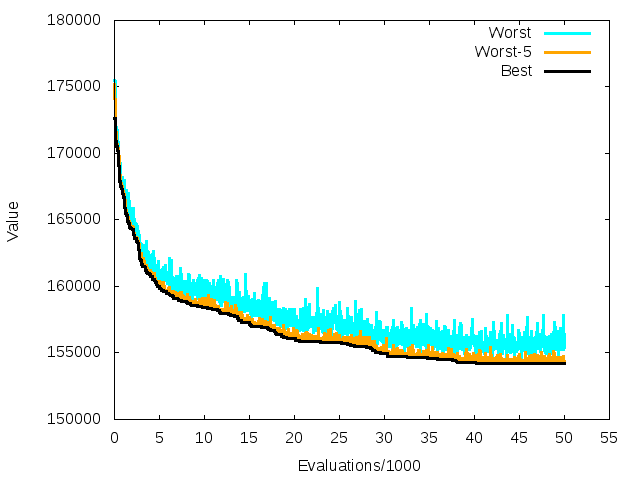
\includegraphics[scale=0.4]{Plots/AGGPos.png} 
			\caption{Gráfica que muestra la evolución de la población en el Algoritmo Genético Generacional con Cruce por Posición.} \label{fig:figura2}
		\end{figure} 
		
		\newpage
		
		\noindent En la gráfica podemos observar que la población converge en etapas tempranas del algoritmo, de forma que es el operador de mutación el encargado de introducir diversidad en la población en etapas posteriores. Tal y como habíamos predicho, el valor de la peor solución oscila durante todo el desarrollo del algoritmo; la cuarta peor solución nos proporciona una mejor medida para determinar la convergencia de la población.
	
	
	
	\FloatBarrier
	
	\subsection{Análisis de resultados del Algoritmo Genético Generacional con cruce OX}
	
	\noindent En la siguiente tabla se encuentran recogidos los datos obtenidos para el Algoritmo Genético Generacional con Cruce OX:

	\begin{table}[!h]
		\centering
		\setlength{\arrayrulewidth}{1mm}
		\setlength{\tabcolsep}{10pt}
		\renewcommand{\arraystretch}{1}
		
		\rowcolors{2}{gray!25}{white}
		\begin{tabular}{ >{\centering\arraybackslash}m{1.3cm}  >{\centering\arraybackslash}m{1.3cm}  >{\centering\arraybackslash}m{2cm}   >{\centering\arraybackslash}m{1.3cm}  >{\centering\arraybackslash}m{1.6cm}  >{\centering\arraybackslash}m{2cm} }
			\hline
			\rowcolor{black}
			\multicolumn{6}{c}{\bf \color{white}{Algoritmo Genético Generacional con Cruce OX}}\\
			\hline
			\rowcolor{gray!50}
			\textbf{Caso} & \textbf{Desv} & \textbf{Tiempo} & \textbf{Caso} & \textbf{Desv} & \textbf{Tiempo} \\
			chr20b & 45.5527 & 0.0622186 & sko100a  & 2.7326 & 0.896222 \\
			chr22a & 15.2762 & 0.0682377 & sko100b  & 2.6029 & 0.902475 \\
			els19 & 22.0427 & 0.0591677 & sko100c  & 3.1175 & 0.913839 \\
			esc32b & 28.0952 & 0.131873 & sko100d  & 3.17752 & 0.910332 \\
			kra30b & 6.90877 & 0.103364 & sko100e  & 3.45156 & 0.899383 \\
			lipa90b & 22.7863 & 0.751808 & tai30  & 9.34051 & 0.103178 \\
			nug25 & 4.13462 & 0.079573 & tai50  & 4.62364 & 0.270896 \\
			sko56 & 3.33275 & 0.290638 & tai60  & 5.66483 & 0.355871 \\
			sko64 & 3.09621 & 0.392527 & tai256  & 1.29891 & 5.45478 \\
			sko72 & 3.26793 & 0.528597 & tho150  & 4.36575 & 1.85704 \\
			\hline
			
		\end{tabular}
		
		\caption{Tabla que contiene los datos asociados al AG Generacional con Cruce OX}
		
	\end{table}
	
	\noindent De igual forma que en el caso anterior el Algoritmo Genético Generacional con Cruce OX proporciona, en la mayoría de las ocasiones, soluciones de calidad en un tiempo reducido, por tanto, podemos concluir que, salvo en algunas excepciones, se trata de un buen método de resolución para el problema de la asignación cuadrática, aunque, una vez más, encontramos casos en los que el método parece no comportarse como se espera de él, sobre todo en los casos de dimensión reducida.
	
	\noindent Podemos también representar en una gráfica los mismos datos que representábamos en el caso anterior para comprobar que este algoritmo parece comportarse de manera muy similar al anterior, lo que es de esperar puesto que comparten la mayoría de operadores.
	
	\begin{figure}[!h]
		\centering
		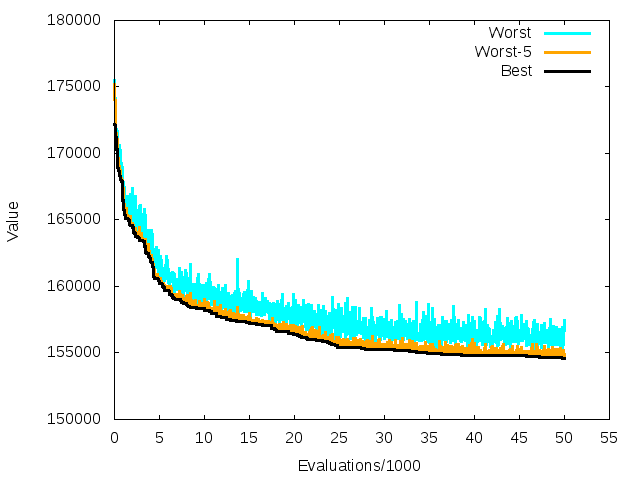
\includegraphics[scale=0.4]{Plots/AGGOX.png} 
		\caption{Gráfica que muestra la evolución de la población en el Algoritmo Genético Generacional con Cruce OX.} \label{fig:figura3}
	\end{figure} 
	
	\FloatBarrier
	
	\subsection{Análisis de resultados del Algoritmo Genético Estacionario con cruce por posición}
	
	\noindent La tabla que recoge los datos obtenidos para el Algoritmo Genético Generacional con Cruce por Posición es la siguiente:\\
	
	\begin{table}[h]
		\centering
		\setlength{\arrayrulewidth}{1mm}
		\setlength{\tabcolsep}{10pt}
		\renewcommand{\arraystretch}{1}
		
		\rowcolors{2}{gray!25}{white}
		\begin{tabular}{ >{\centering\arraybackslash}m{1.3cm}  >{\centering\arraybackslash}m{1.3cm}  >{\centering\arraybackslash}m{2cm}   >{\centering\arraybackslash}m{1.3cm}  >{\centering\arraybackslash}m{1.6cm}  >{\centering\arraybackslash}m{2cm}  }
			\hline
			\rowcolor{black}
			\multicolumn{6}{c}{\bf \color{white}{Algoritmo Genético Estacionario con Cruce por Posición}}\\
			\hline
			\rowcolor{gray!50}
			\textbf{Caso} & \textbf{Desv} & \textbf{Tiempo} & \textbf{Caso} & \textbf{Desv} & \textbf{Tiempo} \\
			chr20b & 41.9669 & 0.0532135 & sko100a  & 3.32759 & 0.644159 \\
			chr22a & 13.8012 & 0.0588647 & sko100b  & 3.00214 & 0.644345 \\
			els19 & 17.0068 & 0.0516091 & sko100c  & 3.62933 & 0.644071 \\
			esc32b & 40.4762 & 0.102095 & sko100d  & 3.38985 & 0.64236 \\
			kra30b & 6.18902 & 0.0871975 & sko100e  & 3.7361 & 0.6509 \\
			lipa90b & 23.1209 & 0.554006 & tai30  & 17.1822 & 0.083847 \\
			nug25 & 4.97863 & 0.0679414 & tai50  & 7.50317 & 0.188142 \\
			sko56 & 3.96773 & 0.23033 & tai60  & 6.04028 & 0.258917 \\
			sko64 & 4.27069 & 0.291898 & tai256  & 1.27122 & 4.18861 \\
			sko72 & 3.86803 & 0.365735 & tho150  & 4.73633 & 1.35778 \\
			\hline
			
		\end{tabular}
		
		\caption{Tabla que contiene los datos asociados al AG Estacionario con Cruce por Posición}
		
	\end{table}
	
	\noindent A la vista de los resultados podemos concluir que, aunque el Algoritmo Genético Estacionario con Cruce por Posición proporciona soluciones de calidad en tiempo reducido, parece comportarse peor que la versión generacional del mismo, además de presentar un leve aumento en el tiempo de ejecución medio. Por otra parte podríamos decir que el algoritmo se comporta mejor que los anteriores en casos de dimensión reducida.
	
	%\noindent Una vez mas podemos representar en una gráfica los mismos datos que en los casos anteriores:
	
	%\begin{figure}[!h]
	%	\centering
	%	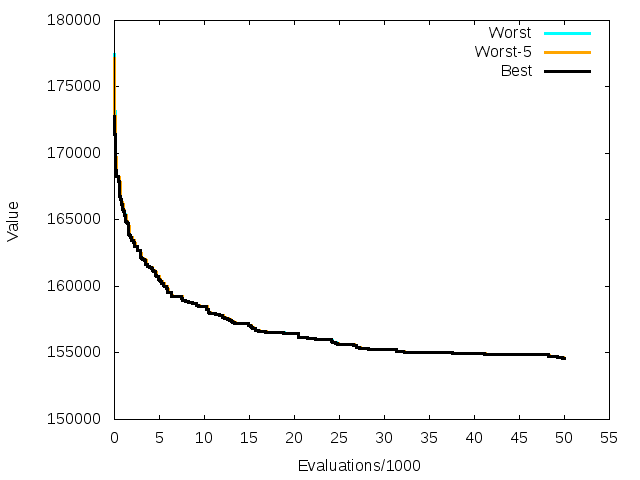
\includegraphics[scale=0.42]{Plots/AGEPos.png} 
	%	\caption{Gráfica que muestra la evolución de la población en el Algoritmo Genético Estacionario con Cruce por Posición.} %\label{fig:figura4}
	%\end{figure} 
	
	%\noindent En esta ocasión vemos que, aunque la población converge en etapas tempranas del algoritmo, el peor elemento 
	
	\subsection{Análisis de resultados del Algoritmo Genético Estacionario con cruce OX}
	
	\noindent La tabla que recoge los datos obtenidos para el Algoritmo Genético Generacional con Cruce por Posición es la siguiente:\\
	
	\begin{table}[h]
		\centering
		\setlength{\arrayrulewidth}{1mm}
		\setlength{\tabcolsep}{10pt}
		\renewcommand{\arraystretch}{1}
		
		\rowcolors{2}{gray!25}{white}
		\begin{tabular}{ >{\centering\arraybackslash}m{1.3cm}  >{\centering\arraybackslash}m{1.3cm}  >{\centering\arraybackslash}m{2cm}   >{\centering\arraybackslash}m{1.3cm}  >{\centering\arraybackslash}m{1.6cm}  >{\centering\arraybackslash}m{2cm}  }
			\hline
			\rowcolor{black}
			\multicolumn{6}{c}{\bf \color{white}{Algoritmo Genético Estacionario con Cruce OX}}\\
			\hline
			\rowcolor{gray!50}
			\textbf{Caso} & \textbf{Desv} & \textbf{Tiempo} & \textbf{Caso} & \textbf{Desv} & \textbf{Tiempo} \\
			chr20b & 47.9373 & 0.0734059 & sko100a  & 3.11206 & 0.919068 \\
			chr22a & 13.3073 & 0.0814037 & sko100b  & 3.18929 & 0.901415 \\
			els19 & 17.3905 & 0.0712997 & sko100c  & 3.52383 & 0.900159 \\
			esc32b & 37.1429 & 0.142177 & sko100d  & 3.26603 & 0.896762 \\
			kra30b & 5.28768 & 0.115615 & sko100e  & 3.79511 & 0.906793 \\
			lipa90b & 22.9082 & 0.760734 & tai30  & 11.2028 & 0.116365 \\
			nug25 & 4.2735 & 0.0933909 & tai50  & 7.84641 & 0.262443 \\
			sko56 & 4.53422 & 0.299718 & tai60  & 5.76926 & 0.361858 \\
			sko64 & 4.37626 & 0.421914 & tai256  & 1.0706 & 5.22044 \\
			sko72 & 3.3923 & 0.533318 & tho150  & 4.46311 & 1.90374 \\
			\hline
			
		\end{tabular}
		
		\caption{Tabla que contiene los datos asociados al AG Estacionario con Cruce OX}
		
	\end{table}
	
	\noindent Viendo los resultados podemos decir que, de igual forma que en el caso anterior, el Algoritmo Genético Estacionario con Cruce OX proporciona, salvo por algunas excepciones, soluciones de calidad para el problema que nos ocupa, aunque con un leve aumento en el tiempo respecto al caso anterior. Sin embargo, la desviación media sí parece mejorar respecto al caso anterior.
	
	\subsection{Análisis de los resultados de los Algoritmos Meméticos}
	
	\subsubsection{Análisis de resultados}
	
	\noindent En comparación con los algoritmos genéticos, los algoritmos meméticos presentan unos resultados excelentes en cuanto a desviación respecto al óptimo se refiere, aunque con una leve pérdida en el tiempo con respecto a los mismos.
	
	\noindent Como cabe esperar, el algoritmo memético que mejores resultados presenta es el de mejora completa de la población. Este algoritmo, aún empleando la mayoría de las evaluaciones disponibles en la búsqueda local, consigue mejorar los resultados proporcionados por los otros dos algoritmos meméticos, que emplean mas evaluaciones en la evolución de la población. Este resultado se debe a la calidad de las soluciones proporcionadas por la búsqueda local. Cabe destacar que, aunque este algoritmo proporciona mejores resultados en desviación, presenta también un leve aumento en el tiempo de ejecución respecto a sus dos competidores.
	
	\noindent Seguido del algoritmo memético de mejora completa encontramos al de mejora parcial aleatoria, que supera al de mejora elitista, esto puede deberse a que, al contrario que el elitista, la mejora parcial aleatoria introduce diversidad en la población, lo que le permite explorar un espacio de soluciones más amplio.
	
	\noindent Podemos representar en una gráfica, de igual forma que hacíamos con los algoritmos genéticos generaciones, los valores de la mejor, peor, y cuarta peor solución para obtener información sobre el comportamiento de la población en cada uno de los algoritmos meméticos.
	
	\begin{figure}[!h]
		\centering
		\begin{minipage}[b]{0.4\textwidth}
			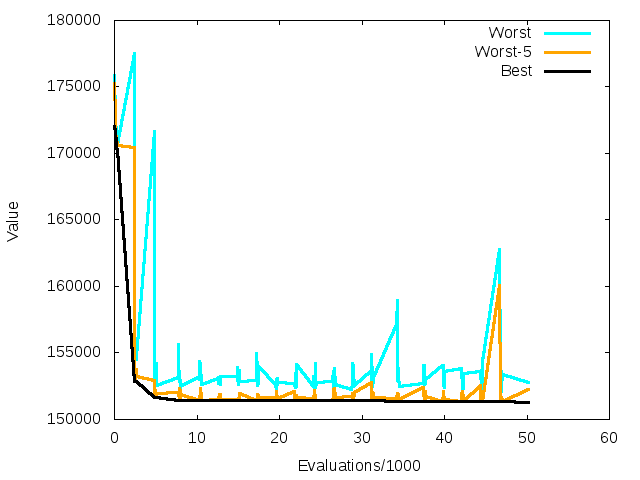
\includegraphics[width=\textwidth]{Plots/AMSub.png}
			\caption{Gráfica que muestra la evolución de la población en el Algoritmo Memético de mejora parcial.}
		\end{minipage}
		\hfill
		\begin{minipage}[b]{0.4\textwidth}
			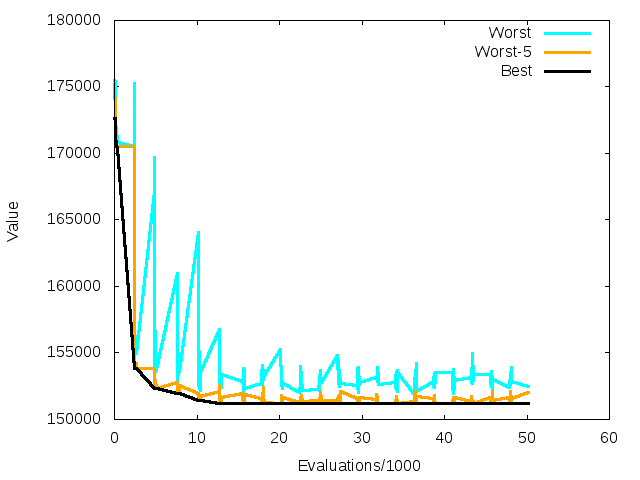
\includegraphics[width=\textwidth]{Plots/AMElite.png}
			\caption{Gráfica que muestra la evolución de la población en el Algoritmo Memético de mejora elitista.}
		\end{minipage}
	\end{figure}
	
	\noindent A la vista de las gráficas podemos decir que los algoritmos se comportan de forma similar. Las oscilaciones en las peores soluciones de deben a que, en las iteraciones en las que se mejora la población, en el caso de la mejora parcial cabe la posibilidad de que la peor solución sea mejorada y deje de ser la peor solución para dar paso a otra solución peor que la anterior; mientras que, en el caso de la mejora elitista vemos que la peor solución tiende a estabilizarse y acercarse a la mejor, esto se debe a que no es posible que la peor solución deje de serlo debido a búsquedas locales, ya que estas solo se aplican a los mejores individuos de la población, de esta forma la peor solución solo puede mejorar al ser reemplazada por otra durante el proceso de reemplazo o mutación.
	
	\begin{figure}[!h]
		\centering
		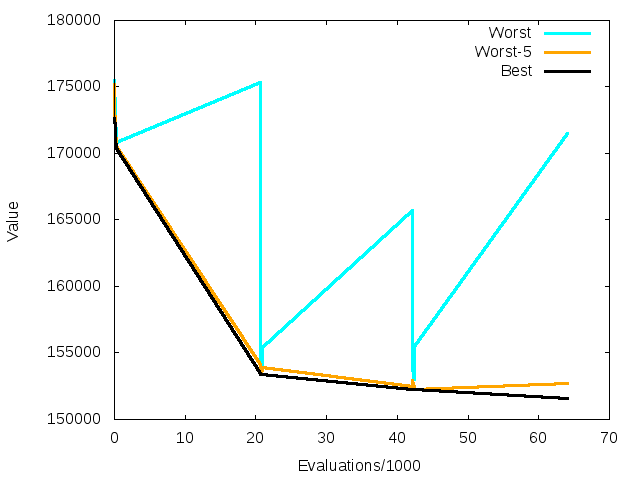
\includegraphics[scale=0.42]{Plots/AMFull.png} 
		\caption{Gráfica que muestra la evolución de la población en el Algoritmo Memético de mejora completa.} \label{fig:figura5}
	\end{figure}
	
	\noindent Dado que en el caso del algoritmo memético de mejora completa se emplean muchas más iteraciones en la búsqueda local  que en los otros dos, no es posible hacer una medición realmente significativa, ya que, al representar el valor frente al número de evaluaciones realizadas se da el caso de que la ``distancia'' entre mediciones es demasiado grande. Aún con esto podemos ver en la gráfica una clara oscilación de la peor solución debido a la pérdida de calidad de esta entre llamadas a la búsqueda local para la misma, mientras que la mejor solución mejora en etapas tempranas del algoritmo y se mantiene relativamente estable.
	
	\subsubsection{Tabla de resultados del Algoritmo Memético con mejora completa}
	
	\noindent La tabla que recoge los datos obtenidos para el Algoritmo Memético con mejora completa:
	
	\begin{table}[!h]
		\centering
		\setlength{\arrayrulewidth}{1mm}
		\setlength{\tabcolsep}{10pt}
		\renewcommand{\arraystretch}{1.2}
		
		\rowcolors{2}{gray!25}{white}
		\begin{tabular}{ >{\centering\arraybackslash}m{1.3cm}  >{\centering\arraybackslash}m{1.3cm}  >{\centering\arraybackslash}m{2cm}   >{\centering\arraybackslash}m{1.3cm}  >{\centering\arraybackslash}m{1.6cm}  >{\centering\arraybackslash}m{2cm}  }
			\hline
			\rowcolor{black}
			\multicolumn{6}{c}{\bf \color{white}{Algoritmo Memético con Mejora Completa}}\\
			\hline
			\rowcolor{gray!50}
			\textbf{Caso} & \textbf{Desv} & \textbf{Tiempo} & \textbf{Caso} & \textbf{Desv} & \textbf{Tiempo} \\
			chr20b & 15.0566 & 0.0342958 & sko100a  & 0.982092 & 1.01435 \\
			chr22a & 4.73684 & 0.041258 & sko100b  & 1.12782 & 1.02969 \\
			els19 & 5.41856 & 0.0313037 & sko100c  & 1.06856 & 1.00132 \\
			esc32b & 10 & 0.0842199 & sko100d  & 1.26277 & 1.02495 \\
			kra30b & 1.43951 & 0.0757131 & sko100e  & 1.23419 & 0.999133 \\
			lipa90b & 21.3346 & 0.89017 & tai30  & 1.89744 & 0.0756545 \\
			nug25 & 0.224359 & 0.0529801 & tai50  & 1.36411 & 0.236681 \\
			sko56 & 1.31058 & 0.2804 & tai60  & 3.32016 & 0.330597 \\
			sko64 & 1.25448 & 0.382895 & tai256  & 0.330001 & 11.4529 \\
			sko72 & 1.12594 & 0.510219 & tho150  & 1.649 & 2.33096 \\
			\hline
			
		\end{tabular}
		
		\caption{Tabla que contiene los datos asociados al AM con mejora completa}
		
	\end{table}
	
	
	\subsubsection{Tabla de resultados del Algoritmo Memético con mejora parcial}
	
	\noindent La tabla que recoge los datos obtenidos para el Algoritmo Memético con mejora parcial:\\
	
	\begin{table}[!h]
		\centering
		\setlength{\arrayrulewidth}{1mm}
		\setlength{\tabcolsep}{10pt}
		\renewcommand{\arraystretch}{1.2}
		
		\rowcolors{2}{gray!25}{white}
		\begin{tabular}{ >{\centering\arraybackslash}m{1.3cm}  >{\centering\arraybackslash}m{1.3cm}  >{\centering\arraybackslash}m{2cm}   >{\centering\arraybackslash}m{1.3cm}  >{\centering\arraybackslash}m{1.6cm}  >{\centering\arraybackslash}m{2cm}  }
			\hline
			\rowcolor{black}
			\multicolumn{6}{c}{\bf \color{white}{Algoritmo Memético con Mejora Parcial}}\\
			\hline
			\rowcolor{gray!50}
			\textbf{Caso} & \textbf{Desv} & \textbf{Tiempo} & \textbf{Caso} & \textbf{Desv} & \textbf{Tiempo} \\
			chr20b & 17.7894 & 0.0361432 & sko100a  & 1.33604 & 0.781477 \\
			chr22a & 6.78363 & 0.0410684 & sko100b  & 1.14107 & 0.767343 \\
			els19 & 11.461 & 0.0369109 & sko100c  & 1.43999 & 0.794057 \\
			esc32b & 14.7619 & 0.0842439 & sko100d  & 1.25742 & 0.791422 \\
			kra30b & 2.08488 & 0.0722008 & sko100e  & 1.40127 & 0.765639 \\
			lipa90b & 21.2198 & 0.632343 & tai30  & 4.91814 & 0.0713379 \\
			nug25 & 0.82265 & 0.0529358 & tai50  & 3.27844 & 0.198651 \\
			sko56 & 1.46497 & 0.234458 & tai60  & 3.5654 & 0.270645 \\
			sko64 & 1.32377 & 0.312339 & tai256  & 0.367375 & 7.52126 \\
			sko72 & 1.27264 & 0.42065 & tho150  & 1.96439 & 1.87782 \\
			\hline
			
		\end{tabular}
		
		\caption{Tabla que contiene los datos asociados al AM con mejora parcial}
		
	\end{table}
	
	\subsubsection{Tabla de resultados del Algoritmo Memético con mejora elitista}
	
	\noindent La tabla que recoge los datos obtenidos para el AM con mejora elitista:\\
	
	\begin{table}[!h]
		\centering
		\setlength{\arrayrulewidth}{1mm}
		\setlength{\tabcolsep}{10pt}
		\renewcommand{\arraystretch}{1.2}
		
		\rowcolors{2}{gray!25}{white}
		\begin{tabular}{ >{\centering\arraybackslash}m{1.3cm}  >{\centering\arraybackslash}m{1.3cm}  >{\centering\arraybackslash}m{2cm}   >{\centering\arraybackslash}m{1.3cm}  >{\centering\arraybackslash}m{1.6cm}  >{\centering\arraybackslash}m{2cm}  }
			\hline
			\rowcolor{black}
			\multicolumn{6}{c}{\bf \color{white}{Algoritmo Memético con mejora elitista}}\\
			\hline
			\rowcolor{gray!50}
			\textbf{Caso} & \textbf{Desv} & \textbf{Tiempo} & \textbf{Caso} & \textbf{Desv} & \textbf{Tiempo} \\
			chr20b & 28.651 & 0.0356483 & sko100a  & 1.37972 & 0.771712 \\
			chr22a & 10.0975 & 0.0412956 & sko100b  & 1.53304 & 0.768565 \\
			els19 & 9.97299 & 0.03414 & sko100c  & 1.06992 & 0.782791 \\
			esc32b & 12.381 & 0.0814054 & sko100d  & 1.32535 & 0.782545 \\
			kra30b & 3.58565 & 0.0786399 & sko100e  & 1.86336 & 0.762292 \\
			lipa90b & 21.6455 & 0.626443 & tai30  & 3.3962 & 0.0762582 \\
			nug25 & 1.78419 & 0.0507658 & tai50  & 3.07605 & 0.189336 \\
			sko56 & 2.07557 & 0.236508 & tai60  & 3.33128 & 0.269062 \\
			sko64 & 1.9341 & 0.307968 & tai256  & 0.371783 & 7.39254 \\
			sko72 & 1.47609 & 0.398982 & tho150  & 1.79966 & 1.86555 \\
			\hline
			
		\end{tabular}
		
		\caption{Tabla que contiene los datos asociados al AM con mejora elitista}
		
	\end{table}
	
	\newpage
	
	\subsection{Análisis de resultados generales}
	
	\noindent La siguiente tabla recoge los resultados medios obtenidos para cada algoritmo:
	
	\begin{table}[h]
		\centering
		\setlength{\arrayrulewidth}{1mm}
		\setlength{\tabcolsep}{10pt}
		\renewcommand{\arraystretch}{1.3}
		
		\rowcolors{2}{gray!25}{white}
		\begin{tabular}{ >{\centering\arraybackslash}m{3.5cm}  >{\centering\arraybackslash}m{2.1cm}  >{\centering\arraybackslash}m{2.7cm} }
			\hline
			\rowcolor{black}
			\textbf{\color{white} Algoritmo} & \textbf{\color{white} Desv} & \textbf{\color{white} Tiempo} \\
			Greedy & 	62,01996  & 4,481808E-05 \\
			BL & 10,45195775  & 0,0467831012 \\
			AGG - Posicion & 9,4154605  & 0,53842018 \\
			AGG - OX & 9,743455  & 0,74514024 \\
			AGE - Posicion & 10,6732155  & 0,554948265  \\
			AGE - OX & 10,389433  & 0,75297976 \\
			AM - (10, 1.0) & 3,8068806  & 1,09386312  \\
			AM - (10, 0.1) & 4,98270875  & 0,78891195 \\
			AM - (10, 0.1 mej) & 5,63749765  & 0,78767248 \\
			\hline
			
		\end{tabular}
		
		\caption{Tabla que contiene los datos asociados al análisis de resultados medios generales}
		
	\end{table}
	
	\noindent La tabla de resultados generales nos permite tener una visión mas general del comportamiento de los algoritmos. Podemos ver que los algoritmos que mejor se comportan respecto a la desviación son, con diferencia, los algoritmos meméticos; esto se debe a que utilizan más información para resolver el problema que los algoritmos genéticos. Por otra parte, estos últimos proporcionan soluciones de cierta calidad, concretamente los generacionales superan a la búsqueda local, aunque no en tiempo, si en desviación.\\
	
	\noindent Respecto a los diferentes operadores de cruce podemos ver que, en el caso de los generaciones se comporta mejor el cruce por posición, mientras que en el caso de los estacionarios es el OX el que mejor actúa, podemos concluir entonces que el mejor comportamiento de uno u otro depende, no solo de la técnica con la que lo combinemos, también de la instancia concreta del problema a la que lo apliquemos\\
	
	\noindent Por último, los métodos no basados en poblaciones. El algoritmo voraz proporciona soluciones en tiempo inmejorable, aunque de baja calidad, mientras que la búsqueda local proporciona soluciones que no tiene que envidiar a las proporcionadas por los genéticos en algunos casos y además en un tiempo menor.
	
\section{Manual de usuario}

	\noindent Junto al código fuente utilizado para el desarrollo de la práctica se incluye un archivo tipo makefile que automatiza el proceso de compilación; este archivo genera un fichero ejecutable para cada uno de los algoritmos, así como un ejecutable general llamado \texttt{mainGeneral} que lanza todos los algoritmos con los parámetros especificados en el guión, es este último el utilizado para tomar las mediciones pertinentes. Además, se incorpora un archivo \texttt{run.sh} que ejecutará el archivo \texttt{mainGeneral} para cada una de las instancias del problema y almacenará el resultado en el directorio \texttt{results} bajo el nombre de \texttt{<nombre\_instancia>.rslt}.
	
	\noindent En la estructura de directorios también se encuentra el directorio \texttt{graphs}, que contiene los datos tomados para la obtención de las gráficas, así como estas mismas.
	

\end{document}

\grid

		\begin{table}[h]
			\centering
			\setlength{\arrayrulewidth}{1mm}
			\setlength{\tabcolsep}{10pt}
			\renewcommand{\arraystretch}{1.5}
			
			\rowcolors{2}{gray!25}{white}
			\begin{tabular}{ >{\centering\arraybackslash}m{1.3cm}  >{\centering\arraybackslash}m{1.3cm}  >{\centering\arraybackslash}m{2cm}   >{\centering\arraybackslash}m{1.3cm}  >{\centering\arraybackslash}m{1.6cm}  >{\centering\arraybackslash}m{2cm}  }
				\hline
				\rowcolor{black}
				\multicolumn{6}{c}{\bf \color{white}{Algoritmo Greedy}}\\
				\hline
				\rowcolor{gray!50}
				\textbf{Caso} & \textbf{Desv} & \textbf{Tiempo} & \textbf{Caso} & \textbf{Desv} & \textbf{Tiempo} \\
				chr20b &   &   & sko100a  &   &   \\
				chr22a &   &   & sko100b  &   &   \\
				els19 &   &   & sko100c  &   &   \\
				esc32b &   &   & sko100d  &   &   \\
				kra30b &   &   & sko100e  &   &   \\
				lipa90b &   &   & tai30  &   &   \\
				nug25 &   &   & tai50  &   &   \\
				sko56 &   &   & tai60  &   &   \\
				sko64 &   &   & tai256  &   &   \\
				sko72 &   &   & tho150  &   &   \\
				\hline
				
			\end{tabular}
			
		\end{table}